\begin{frame}{Le concept de Bolter et Grusin}
    \begin{columns}[T,onlytextwidth]
\column{0.50\linewidth}
\small
\begin{itemize}
    \item Ouvrage de référence : Jay David Bolter, Richard Grusin,\textit{Remediation : Understanding New Media}
    \item Dans la relation intermédiale: une logique évolutive des médias = c'est dans la nature de tout nouveau média que de plagier son aîné.
    \item Remédiation = une répétition, la trace d’un ancien médium dans un nouveau.
\end{itemize}

\column{0.50\linewidth}
\centering
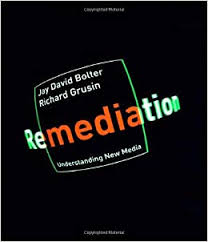
\includegraphics[width=.70\columnwidth]{Images/remediation.jpeg}
\end{columns}
\textrightarrow{} Le public aime ce qui lui est familier.
\end{frame}

\begin{frame}{La relation intermédiale}
    \begin{block}{}
        \centering
        \small{\textit{L’émergence d’un nouveau média conduit également à une transformation de la forme prise par les médias existants. Pour comprendre cela, il est important de ne pas adopter une définition essentialiste de ce que sont les médias. Au contraire, il s’agit de les considérer comme des formes modulable sans cesse en cours de (re)configuration.}\\
        \textbf{Remy Besson, "\textit{Prolégomène pour une définition de l'intermédialité}"}}
    \end{block}
    \textrightarrow{} Nature hétérogène des médias.
\end{frame}

\begin{frame}{La \textit{mimesis} médiatique : comment mieux "médier" le réel}
    Comment médier le monde? Comment donner accès au réel?

    \begin{block}{Deux stratégies possibles}
        \begin{itemize}
            \item Immédiateté (\textit{immediacy})
            \item Hypermédiateté (\textit{hypermediacy})
        \end{itemize}
    \end{block}
\end{frame}

\begin{frame}{\textit{Immediacy} : la logique de la "transparence"}
    Consiste à donner une meilleure impression de "transparence".\\
    \textrightarrow{} Faire oublier l'interface: pas de boutons, de fenêtres, de scroll-barres, ni même d'icônes.\\
    \textrightarrow{} L'utilisateur.rice n'est plus conscient de se confronter à un support.
\end{frame}

\begin{frame}{\textit{Hypermediacy} : la logique de l'emprunte médiatique (car "Le médium, c'est le message")}
    Consiste à mettre en avant le processus de médiation.\\ 
    \textrightarrow{} "Le médium, c'est le message" = la forme de l'interface (médium) a un impact sur le message.\\
    \textbf{Exemple:} Les dossiers et fichiers sur notre ordinateur miment un bureau avec des dosiers et fichiers.
\end{frame}

\begin{frame}{Du design d'interface...}
\textbf{Quelle interface offre le livre ?}\\
\vspace{2em} 

Le livre est un \textbf{objet de design}. \\
\vspace{2em}
\textbf{Design} =  activité créatrice pour déterminer des propriété formelles des objets que l'on veut reproduire industriellement. (Maldonaclo - 1961, Venise. Définition adoptée par l'SICSID (Conseil International des Sociétés de Design Industriel))\\
\textrightarrow{} Pensé pour faciliter son utilisation.

\end{frame}

\begin{frame}{... à l'histoire des grands medias}
    \begin{itemize}
        \item La remédiation de Bolter et Grusin a été d'abord conceptualisée pour penser les nouvelles technologies
        \item Application à tous les medias et les arts, depuis l'antiquité
    \end{itemize}
\end{frame}

\begin{frame}{Hypermédiateté et immédiateté : une opposition si simple ?}
    Hypermédiateté, c'est-à-dire cette dimension médiatique surjouée, est prépondérante. Pourquoi ? 
    \begin{itemize}
        \item L'expérience de lecture profonde ne doit pas être parasitée par un dispositif trop complexe.
        \item Faire en sorte que les lecteur.rices/spectateur.rices s'approprient l'objet.
    \end{itemize}
\centering
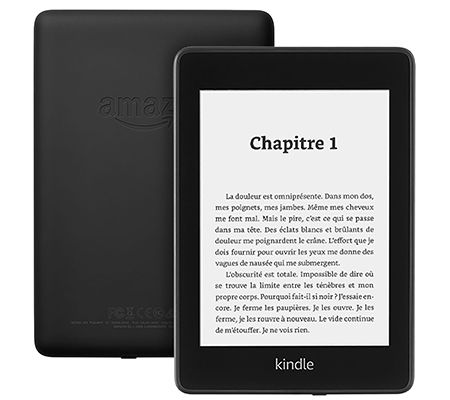
\includegraphics[width=4cm]{Images/kindle-paperwhite-2018-wifi_dcc6d79033e1f191__450_400.jpg}
\end{frame}

\begin{frame}{Le "livre numérique" n'existe pas...}
    \begin{itemize}
        \item "Adaptation" de l'imprimé à un nouveau mode de consultation/diffusion numérique= livres homothétiques;
        \item Propositions techniques et conceptuelles natives numériques (livres-appli par exemple);
        \item Production hybride: complémentarité imprimé et numérique, PAO, web to print.
    \end{itemize}
\end{frame}
